\documentclass{article}
\usepackage{graphicx} % Required for inserting images
\usepackage{amsmath}

% Used for Images
\usepackage{float}

% Used for Table
\usepackage{longtable}

\usepackage{hyperref}


% For R code Syntax
\usepackage{listings}
\usepackage{xcolor}
\definecolor{commcolor}{rgb}{0,0.6,0}
\definecolor{keywordcolor}{rgb}{0,0,1}
\definecolor{stringcolor}{rgb}{0.58,0,0.82}
\lstset{
    language=R,
    basicstyle=\small\ttfamily,
    commentstyle=\color{commcolor},
    keywordstyle=\color{keywordcolor},
    stringstyle=\color{stringcolor},
    breaklines=true,
    frame=single,
    showstringspaces=false,
}

\title{STA304: Exploratory Data Analysis Report\\
\large Student Confidence in the Current Job Market}
\author{Saleena Qureshi, Alisyee Aguirre Coward, Solomon Ador-Dionisio,\\ 
Tanya Misra, and Krish Mehta}
\date{October 25 2026}

\begin{document}
\maketitle
\section{Summary Statistics}
\subsection{Tables for Values}
Note that all of our data is categorical, thus there is no quantitative variables.
% Qualitative Table
\begingroup
    \small
    \setlength{\tabcolsep}{4pt}
    \begin{longtable}{llcccc}
    \caption{Qualitative Variables}\label{tab:qualit_table}\\
    \hline
    Variable & Value & N & Raw \% & Valid \% & Cumulative \% \\ \hline
    \endfirsthead

        % Saleena
        Citizenship Status & Domestic & 34 & 55.74 & 55.74 & 55.74\\
       & International &  27 & 44.26 & 44.26 & 100.00\\
       & (NA) & 0 & 0.00 & (NA) & (NA)\\ \\

        % Solomon
       Year of Study & First Year & 0 & 0.00 & 0.00 & 0.00\\
       & Second Year & 0 & 0.00 & 0.00 & 0.00\\
       & Third Year & 39 & 63.93 & 63.93 & 63.93\\
       & Fourth Year & 18 & 29.51 & 29.51 & 93.44\\
       & Fifth Year or Higher & 4 & 6.56 & 6.56 & 100.00\\
       & (NA) & 0 & 0.00 & (NA) & (NA)\\\\

       % Saleena
       LinkedIn Connections & 0 - 100 & 28 & 45.90 & 62.22 & 62.22\\
       & 100 - 200 & 5 & 8.20 & 11.11 & 73.33\\
       & 200 - 300 & 1 & 1.64 & 2.22 & 75.56\\
       & 300 - 400 & 3 & 4.92 & 6.67 & 82.22\\
       & 400 - 500 & 1 & 1.64 & 2.22 & 84.44\\
       & 500+ & 7 & 11.48 & 15.56 & 100.00\\
       & (NA) & 16 & 26.23 & (NA) & (NA)\\ \\
        
       % Alisyee
        Job Security Confidence & Strongly Agree & 7 & 11.48 & 11.48 & 11.48 \\
        & Agree & 6 & 9.84 & 9.84 & 21.31 \\
        & Slightly Agree & 10 & 16.39 & 16.31 & 37.70 \\
        & Neutral & 8 & 13.11 & 13.11 & 50.82 \\
        & Slightly Disagree & 17 & 27.87 & 27.87 & 78.69 \\
        & Disagree & 9 & 14.75 & 14.75 & 93.44 \\
        & Strongly Disagree & 4 & 6.56 & 6.56 & 100.00 \\
        & (NA) & 0 & 0.00 & (NA) & (NA)\\\\

        Professional Network Confidence & Strongly Agree & 4 & 6.56 & 6.56 & 6.56 \\
        & Agree & 6 & 9.84 & 9.84 & 16.39 \\
        & Slightly Agree & 7 & 11.48 & 11.48 & 27.87 \\
        & Neutral & 14 & 22.95 & 22.95 & 50.82 \\
        & Slightly Disagree & 8 & 13.11 & 13.11 & 63.93 \\
        & Disagree & 13 & 21.31 & 21.31 & 85.25 \\
        & Strongly Disagree & 0 & 14.75 & 14.75 & 100.00 \\
        & (NA) & 0 & 0.00 & (NA) & (NA)\\\\

        % Krish
        Necessary Skills & Strongly Agree & 4 & 6.56 & 6.56 & 6.56 \\
        & Agree & 15 & 24.59 & 24.59 & 31.15 \\
        & Slightly Agree & 10 & 16.39 & 16.39 & 47.54 \\
        & Neutral & 10 & 16.39 & 16.39 & 63.93 \\
        & Slightly Disagree & 9 & 14.75 & 14.75 & 78.69 \\
        & Disagree & 13 & 21.31 & 21.31 & 100.00 \\
        & Strongly Disagree & 0 & 0.00 & 0.00 & 100.00\\
        & (NA) & 0 & 0.00 & (NA) & (NA)\\\\

        Abundant Opportunities & Strongly Agree & 1 & 1.64 & 1.64 & 1.64 \\
        & Agree & 8 & 13.11 & 13.11 & 14.75 \\
        & Slightly Agree & 9 & 14.75 & 14.75 & 29.51 \\
        & Neutral & 17 & 27.87 & 27.87 & 57.38 \\
        & Slightly Disagree & 9 & 14.75 & 14.75 & 72.13 \\
        & Disagree & 13 & 21.31 & 21.31 & 93.44 \\
        & Strongly Disagree & 4 & 6.56 & 6.56 & 100.00 \\
        & (NA) & 0 & 0.00 & (NA) & (NA) \\
        
        
    \hline
    \end{longtable}
\endgroup

    % Brief comment about the Table 1
    

            
\subsection{Observations of Distributions}
Our 61 students were mostly third-year (63.93\%), with a fairly even domestic/international split. LinkedIn connections were generally low, with 62.22\% of valid responses reporting under 100 and 26.23\% missing. Students were mostly neutral or slightly disagreeing about job security and job opportunities, but 47.54\% felt they had the skills employers want, suggesting greater confidence in their abilities than in the job market.

% RQ 1
\section{Research Question 1: Comparisons of means} % Saleena, Krish
\textbf{Research Question:} \textit{How does job market confidence differ between international and domestic students?}

\subsection{Data Visualization (Graph or Table)}
% Graph for RQ1
\begin{figure}[H]
    \centering
    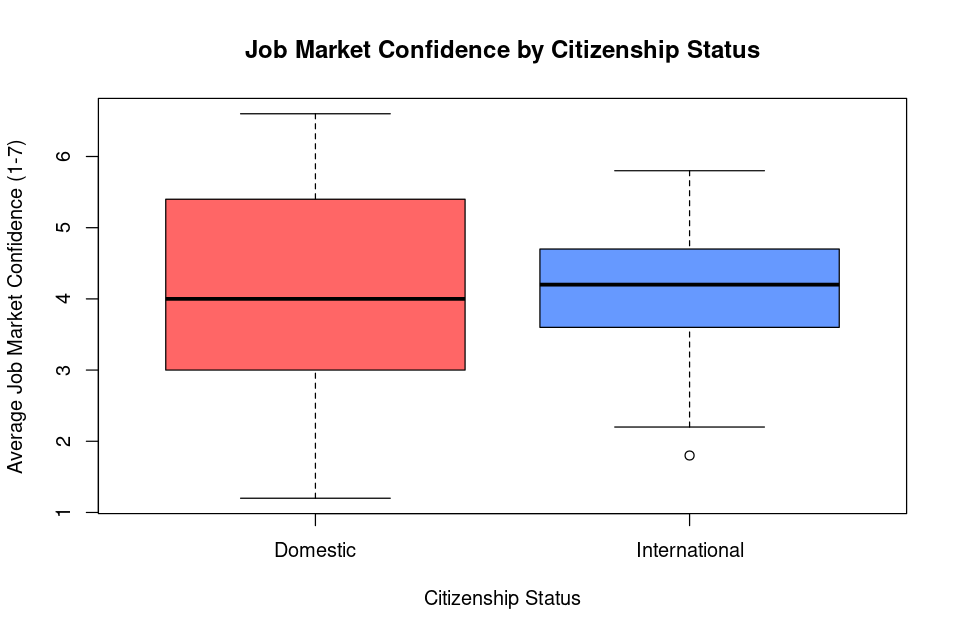
\includegraphics[width=1\linewidth]{RQ1Graph.png}
    \caption{Barplot showcasing the distribution of students’ confidence in the current job market based on whether they were domestic or international. The averages appear to be nearly the same, with Domestic students having a greater spread.}
    \label{fig:rq3}
\end{figure}

\subsection{Checking Model Assumptions}
% Checking Model Assumptions for RQ1
\begin{figure}[H]
    \centering
    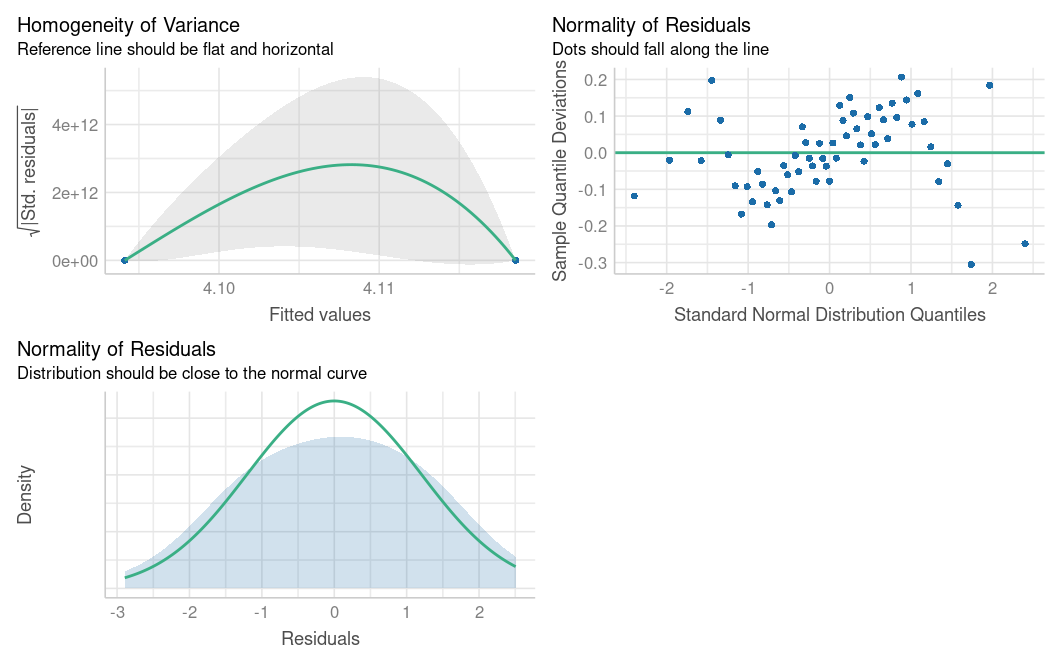
\includegraphics[width=1\linewidth]{RQ1MA.png}
    \caption{Checking the model assumptions of linear regression using the performance package.}
    \label{fig:rq3}
\end{figure}
The QQ plot and Normality of Residuals plot closely follow a normal distribution, thus we can assume the normality assumption holds. The Homogeneity of Variances is unclear, thus we proceed with a Welch's t-test to compare means. This is also backed up by the box plot (Figure 1) where the spreads of the two groups are different, thus implying unequal variances.

\subsection{Statistical Tests and Interpretations}

Effect sizes were labelled following Cohen's (1988) recommendations.\\

The Welch Two Sample t-test testing the difference of Confidence by Status (mean in group Domestic = 4.09, mean in group International = 4.12) suggests that the effect is negative, statistically not significant, and very small (difference = -0.02, 95\% CI [-0.63, 0.58], t(58.55) = -0.08, p = 0.936; Cohen's d = -0.02, 95\% CI [-0.53, 0.49]). Thus, there is not enough evidence to conclude that job market confidence differs between domestic and international students in this sample.


% RQ 2
\section{Research Question 2: Multiple Linear Regression} % Tanya, Alisyee
\textbf{Research Question:} \textit{How strongly does the number of internships/work experience, GPA, and number of followers on LinkedIn influence student confidence?}
\subsection{Data Visualization (Graph or Table)}
% Graph for RQ2
\begin{figure}[H]
    \centering
    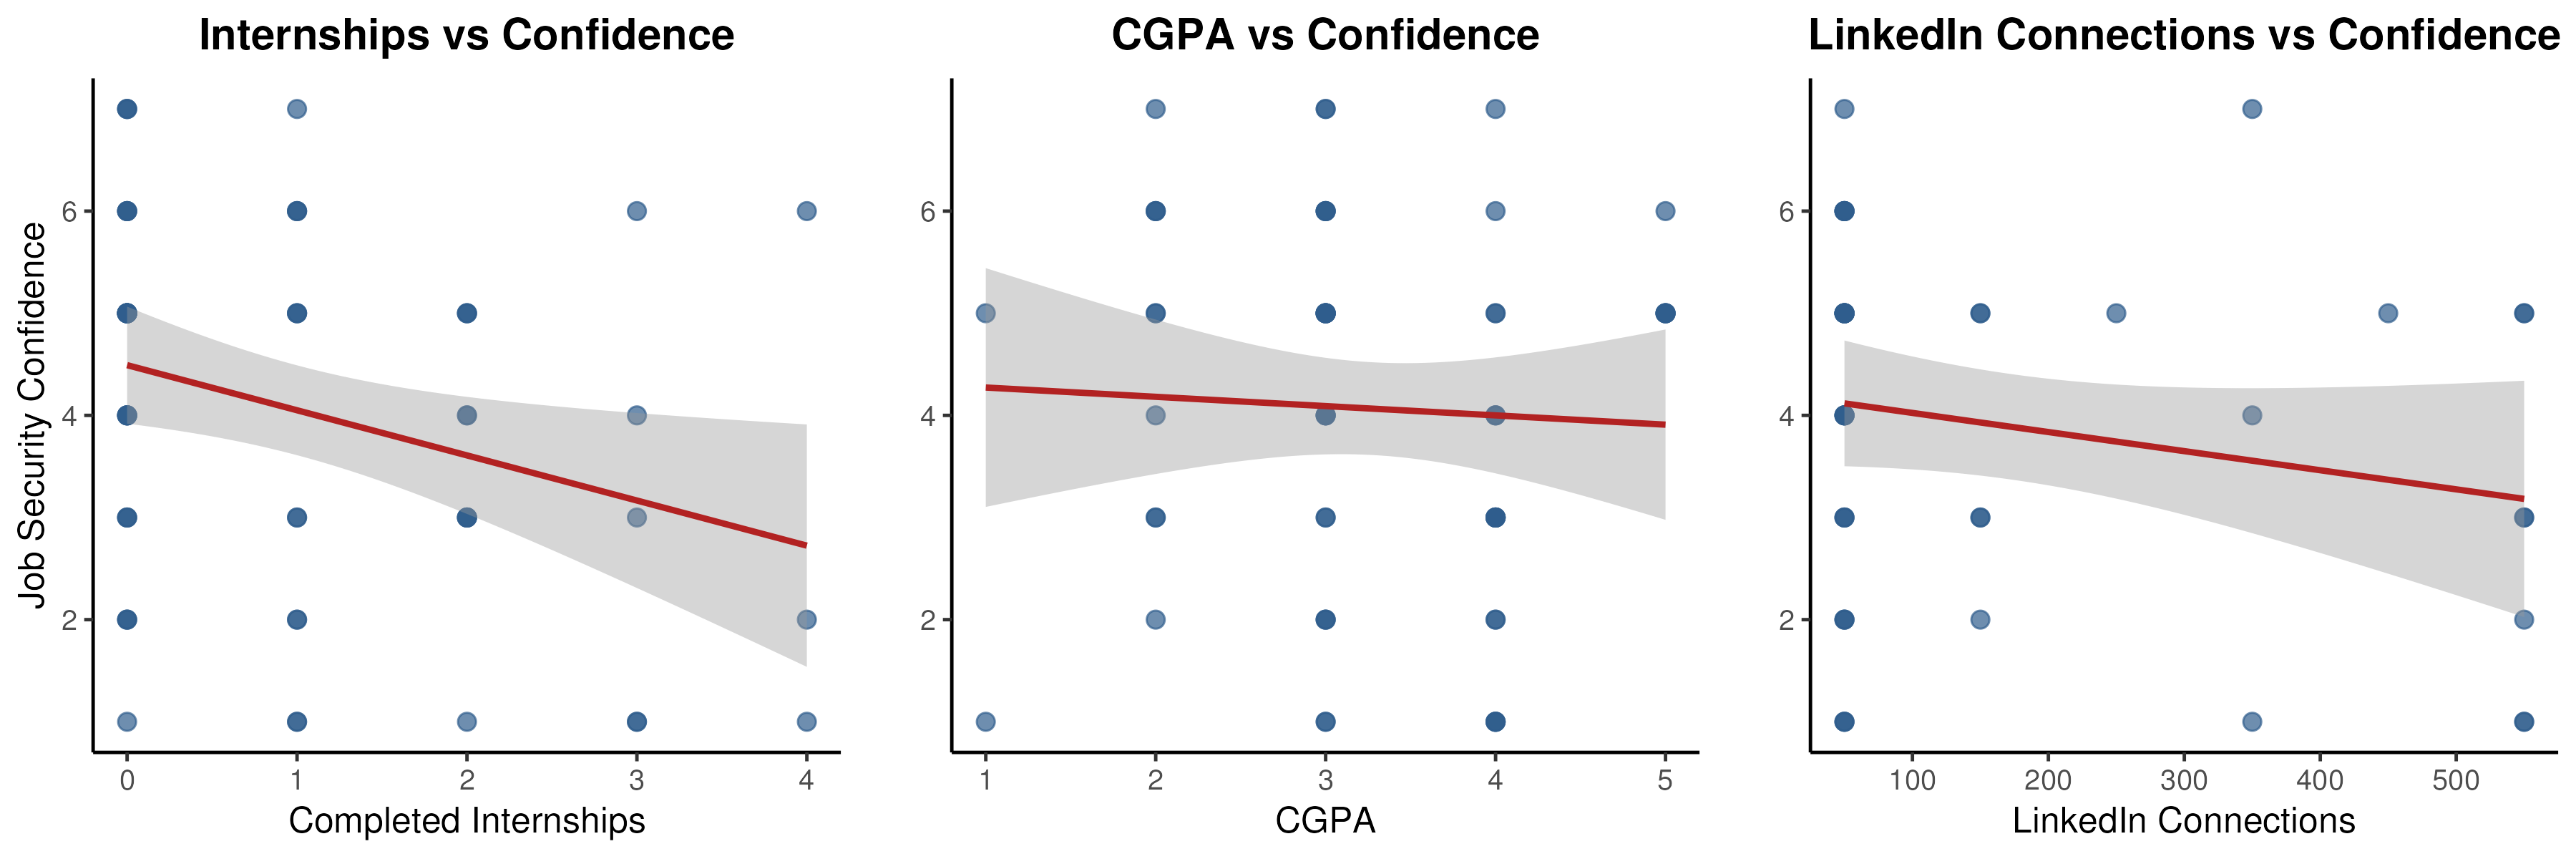
\includegraphics[width=1\linewidth]{RQ2Graph.png}
    \caption{Scatter plots showcasing the individual linear relationships between Student Confidence (measured by Job Security) and three predictors: Completed Internships, CGPA, and LinkedIn Connections, each fitted with a simple linear regression trendline.}
    \label{fig:rq2_scatters}
\end{figure}

\subsection{Checking Model Assumptions}
\begin{figure}[H]
    \centering
    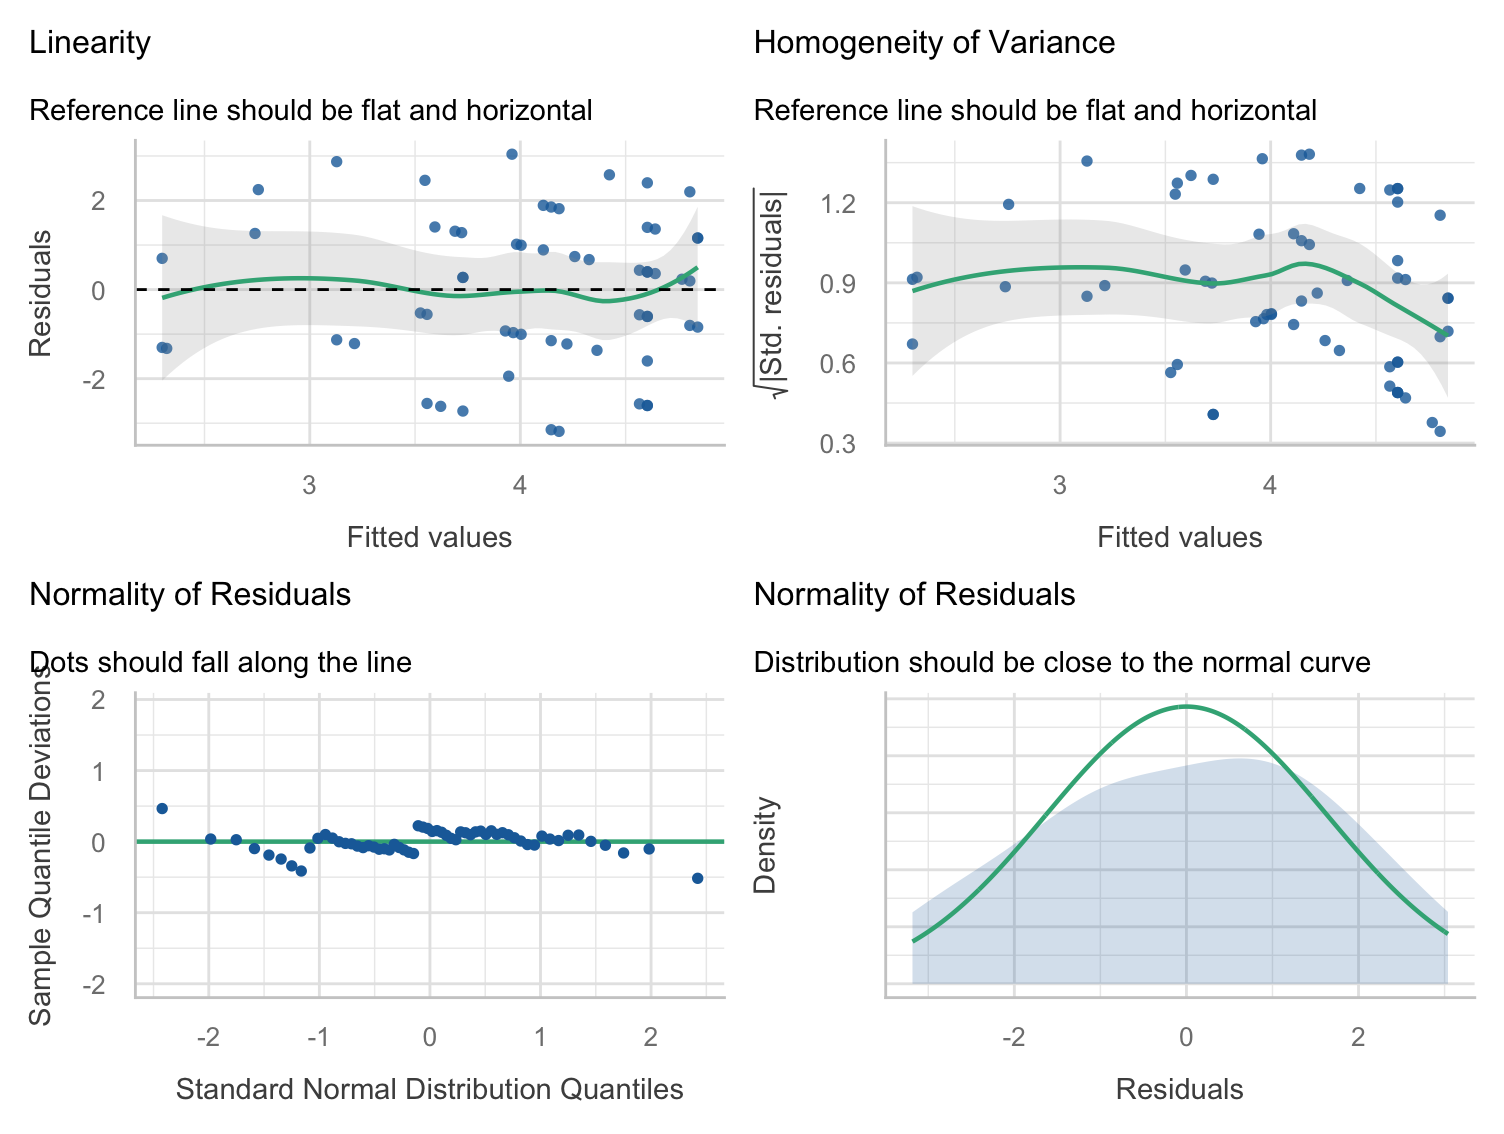
\includegraphics[width=1\linewidth]{RQ2MA.png}
    \caption{Checking the model assumptions of multiple linear regression using the performance package.}
    \label{fig:rq2}
\end{figure}

The performance diagnostic indicates that linearity is satisfied and there are small deviations in homogeneity of variance and normality of the residuals. We may proceed with an OLS inference. \\

\subsection{Statistical Tests and Interpretations}
We fitted a model, using OLS, to predict job security with completed internships, cgpa, and linkedin connections. We notice there is a significant moderate proportion of variance in our ($y$) job security variable. The p-value, $p = 0.035$, falls below the $\alpha = 0.05$. We can reject the null hypothesis and conclude that the predictors provide a better fit than the intercept only model. \\

When observing the individual predictors, we notice that the number of internships has a statistically significant and negative relationship ($\beta_1 = -0.042$, $p = 0.025$) with job security confidence.
CGPA showed no statistically significant relationship with job security confidence ($\beta_1 = -0.04$, $p = 0.876$).
Linkedin Connections has a negative relationship but was also statistically non-significant ($\beta_1 = -0.20$, $p = 0.095$).


% RQ 3
\section{Research Question 3} % Solomon
\textbf{Research Question:} \textit{What proportion of students believe their degree has prepared them for the workforce?}
\subsection{Data Visualization (Graph or Table)}
% Graph for RQ3
\begin{figure}[H]
    \centering
    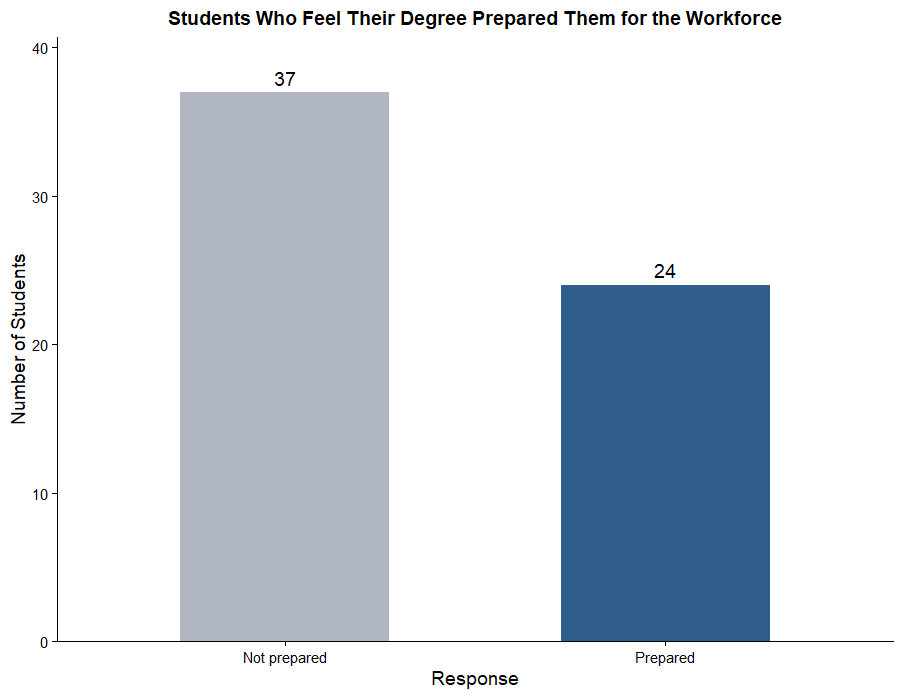
\includegraphics[width=1\linewidth]{RQ3Graph.png}
    \caption{Bargraph showcasing preparedness among the students where strongly, moderately, and slightly prepared are all considered as prepared. It appears that less students feel their degree has prepared them for the workforce.}
    \label{fig:rq3}
\end{figure}

\subsection{Checking Model Assumptions}
For a one-sample $z$-test for a proportion the following conditions must hold:
\begin{itemize}
    \item \textbf{Random sample:} The data must come from a random sample of the
    population. We collected the survey responses from a random sample of
    students in STA302H5, so this condition is satisfied.
    \item \textbf{Independence:} Each student's response must be independent of
    the others. Each student completed the survey individually, and our sample
    is less than 10\% of the student population, so this condition is satisfied.
    \item \textbf{Binary outcome:} Each response must fall into one of two
    categories. We coded responses as ``prepared'' (strongly, moderately or
    slightly prepared) or ``not prepared'' (all other responses), so this
    condition is satisfied.
    \item \textbf{Success-failure condition:} The sampling distribution of
    $\hat{p}$ is approximately normal if $np_0 \geq 10$ and
    $n(1 - p_0) \geq 10$. With $n = 61$ and $p_0 = 0.5$, we have
    $np_0 = n(1 - p_0) = 30.5 \geq 10$, so this condition is satisfied.
\end{itemize}

\subsection{Statistical Tests and Interpretations}
The one-sample z-test testing whether the proportion of students who feel prepared is greater than 0.5 (sample proportion = 0.39, 24 of 61) suggests that the proportion is below the null value and statistically not significant (difference = -0.11, 95\% CI [0.30, 1.00], z = -1.66, p = 0.952). We fail to reject the null hypothesis.

\n This means there is no evidence that more than half of students believe their degree has prepared them for the workforce; in our sample, only 39.3\% did. This suggests that students in our sample do not generally feel that their degree has prepared them for the workforce.


% R code
\newpage
\appendix
\section{Appendix}
\begin{lstlisting}[language=R]
# All packages used
library(easystats)
library(ggplot2)
\end{lstlisting}


% This is the code to display the Summary Statistics for all columns
\begin{lstlisting}[language=R]
# Code to display the Summary Statistics for all columns
data <- read.csv("processed_studentresponses.csv")
dataYear.of.Study<-factor(data$Year.of.Study, levels = 1:5)
data_tabulate(data, select = -studentID, collapse = TRUE)
\end{lstlisting}

% This is the code for RQ1
Code for the Research Question 1
\begin{lstlisting}[language=R]
library(easystats)

df <- read.csv("processed_studentresponses.csv")

# 0 = Domestic, 1 = International
df$Status <- factor(df$Citizenship.Status, levels = c(0, 1), labels = c("Domestic", "International"))

# Job market confidence is the average of the five confidence questions
df$Confidence <- rowMeans(df[, c("Necessary.Skills", "Abundant.Opportunities",
                                 "Job.Security", "Professional.Network",
                                 "Workforce.Preparedness")])

# Creating the box plots
describe_distribution(df$Confidence[df$Status == "Domestic"])
describe_distribution(df$Confidence[df$Status == "International"])

boxplot(Confidence ~ Status, data = df,
        main = "Job Market Confidence by Citizenship Status",
        xlab = "Citizenship Status",
        ylab = "Average Job Market Confidence (1-7)",
        col = c("#FF6666", "#6699FF"))

# Checking model assumptions
model <- lm(Confidence ~ Status, data = df)
check_model(model, check = c("qq", "normality", "homogeneity"))

# Statistical test (Welch t-test)
res <- t.test(Confidence ~ Status, data = df)
report(res)
\end{lstlisting}

% This is the code for RQ2
Code for the Research Question 2
\begin{lstlisting}[language=R]
# 1. Completed Internships vs Job Security
p1 <- ggplot(df, aes(x = Completed.Internships, y = Job.Security)) +
  geom_point(color = "#2F5D8C", alpha = 0.7, size = 2.5) +
  geom_smooth(method = "lm", color = "#B22222", se = TRUE) +
  labs(title = "Internships vs Confidence",
       x = "Completed Internships",
       y = "Job Security Confidence") +
  theme_classic(base_size = 12) +
  theme(plot.title = element_text(face = "bold", hjust = 0.5))

# 2. CGPA vs Job Security
p2 <- ggplot(df, aes(x = CGPA, y = Job.Security)) +
  geom_point(color = "#2F5D8C", alpha = 0.7, size = 2.5) +
  geom_smooth(method = "lm", color = "#B22222", se = TRUE) +
  labs(title = "CGPA vs Confidence",
       x = "CGPA",
       y = "") +
  theme_classic(base_size = 12) +
  theme(plot.title = element_text(face = "bold", hjust = 0.5))

# 3. LinkedIn Connections vs Job Security
p3 <- ggplot(df, aes(x = LinkedIn.Connections, y = Job.Security)) +
  geom_point(color = "#2F5D8C", alpha = 0.7, size = 2.5) +
  geom_smooth(method = "lm", color = "#B22222", se = TRUE) +
  labs(title = "LinkedIn Connections vs Confidence",
       x = "LinkedIn Connections",
       y = "") +
  theme_classic(base_size = 12) +
  theme(plot.title = element_text(face = "bold", hjust = 0.5))

grid.arrange(p1, p2, p3, ncol = 3)

# Checking model assumptions 

# Conducting statistical tests (F-test, T-test)
model_rq2 <- lm(Job.Security ~ Completed.Internships + CGPA + LinkedIn.Connections, data = df)
report::report(model_rq2)


\end{lstlisting}

% This is the code for RQ3
Code for the Research Question 3
\begin{lstlisting}[language=R]
# Combine Prepared and Not prepared data
data$PreparedBin <- factor(ifelse(data$Workforce.Preparedness <= 3, "Prepared", "Not prepared"),
                           levels = c("Not prepared", "Prepared"))

# Bargraph of Preparedness for the Workforce
ggplot(data, aes(x = PreparedBin, fill = PreparedBin)) +
  geom_bar(width = 0.55) +
  geom_text(stat = "count", aes(label = after_stat(count)), vjust = -0.5, size = 5) +
  scale_fill_manual(values = c("Not prepared" = "#B0B7C3", "Prepared" = "#2F5D8C")) +
  scale_y_continuous(expand = expansion(mult = c(0, 0.1))) +
  labs(title = "Students Who Feel Their Degree\nPrepared Them for the Workforce",
       x = "Response",
       y = "Number of Students") +
  theme_classic(base_size = 14) +
  theme(plot.title = element_text(hjust = 0.5, face = "bold", size = 14),
        legend.position = "none")

# Computing One-sample z-test for a proportion: H0: p = 0.5 vs H1: p > 0.5
x <- sum(data$PreparedBin == "Prepared")
n <- nrow(data)

res <- prop.test(x, n, p = 0.5, alternative = "greater", correct = FALSE)
res

p_hat <- x / n
z <- (p_hat - 0.5) / sqrt(0.5 * 0.5 / n)
z
\end{lstlisting}

Overleaf Link: \url{https://www.overleaf.com/project/6adaa1e66c5da9bb3a9c6743/share#600756e84293c66025d2bbb1e647e98a8a5af2895bfa89d0}



\end{document}
